\documentclass[12pt,a4paper]{scrartcl}
\usepackage[utf8]{inputenc}
\usepackage[english]{babel}
\usepackage[T1]{fontenc}
% go to the top of figure instead to caption when following links
\usepackage{subcaption}

\usepackage{icomma}
\usepackage[
    locale = DE,
    space-before-unit=true,
    per-mode = symbol
]{siunitx}
\usepackage{gensymb}

\setlength{\marginparwidth}{2cm}
\usepackage{todonotes}

\usepackage[
    breaklinks=true,
    colorlinks=true,
    linkcolor=blue,
    urlcolor=blue,
    citecolor=blue
]{hyperref} % creates reference links
\usepackage{caption} % go to top of figure
\usepackage{multirow}
\usepackage{tabularx}
\usepackage{booktabs}
\usepackage{biblatex}
\usepackage{csquotes}
\addbibresource{bibliography.bib}

\usepackage{amsfonts,amsmath,amssymb}
\usepackage{textcomp} %\textper(ten)thousand
\usepackage{bm} % for boldface vectors

\usepackage{xcolor}
%[dvipsnames]

\usepackage{pdfpages} % include pdfs
\usepackage{graphicx} % include images
\usepackage{placeins} % \FloatBarrier
\usepackage{pgf} % include pgf plots (matplotlib) -> latex fonts

\usepackage{animate}

% \usepackage{minted} % code blocks
\usepackage{listings}
\definecolor{keywords}{rgb}{0.80, 0.25, 0.18}
\definecolor{comments}{rgb}{0.24,0.48,0.48}     % comments
\definecolor{codegray}{rgb}{0.5,0.5,0.5}
\definecolor{codepurple}{rgb}{0.58,0,0.82}
\definecolor{backcolour}{rgb}{0.85,0.85,0.85}
\definecolor{aqua}{cmyk}{0.65,0,0.23,0}         % class types
\definecolor{lavender}{cmyk}{0,0.42,0,0.1}      % conditionals
\definecolor{self}{rgb}{76,0.53,0.06}           % conditionals


\lstdefinestyle{python}{
    language=Python,
    frame=tbl,
    backgroundcolor=\color{backcolour},  
    basicstyle=\ttfamily\scriptsize,
    keywordstyle=\color{keywords},
    % identifierstyle=\color{blue},
    stringstyle=\color{codepurple},
    commentstyle=\color{comments},
    numberstyle=\tiny\color{codegray},
    breakatwhitespace=false,         
    breaklines=false,                 
    captionpos=b,                    
    keepspaces=true,                 
    numbers=left,                    
    numbersep=5pt,                  
    showspaces=false,                
    showstringspaces=false,
    showtabs=false,                  
    tabsize=4,
    emph={self},
    emphstyle =\color{self}
}

% \lstset{style=python_style}
\usepackage{inconsolata}

\graphicspath{{figures/}}
\makeatletter
\def\input@path{{figures/}}
\makeatother

\author{
    Jakob Floß\footnote{\href{mailto:jakob.floss@student.uibk.ac.at}
    {jakob.floss@student.uibk.ac.at}}
}
    
\title{Reinforcement Learning\\ - Applied to a Maze}

\begin{document}
\titlehead{
\includegraphics[width=5cm]{logo.png}}
\maketitle
% \section*{Abstract}

\thispagestyle{empty}
\newpage

% --- TABLE OF CONTENTS ----------------------------------------------------------------------------
\tableofcontents
\thispagestyle{empty}
\newpage

% --- INTRODUCTION ---------------------------------------------------------------------------------
\section{Introduction to Reinforcement Learning}
\label{sec:intro}

Machine Learning is a powerful tool.
It can be used to automate tasks.
Consider processing a hand-filled form for a bank transfer.
With image recognition the letters of the boxes can be analyzed and the form
can be digitized. The training could be done via supervised learning, as shown
in the lecture.
But what about more complex systems where providing such labeled learning sets
are difficult or even impossible to produce?

Reinforcement learning is one option to tackle such kinds of problems.
How? It lets an agent interact with an environment via action.
Then the agent will get rewards based on his actions.
From this he will learn in a way, maximizing the cumulative reward.

In the following I will follow a tutorial \cite{tutorial} found on Medium.\\

For the example of solving a maze the environment will be the maze and its logic
implemented in a python class.
The agent will be trying to solve this maze in an iterative way, learning from
his previous attempts.

In order to explain the two entities involved in this case, let's take a
closer look at their implementations.

% --- Code Implementation --------------------------------------------------------------------------
\section{Code Implementation}
\label{sec:implementation}

Generally the code is split into three (productive) parts:
\begin{itemize}
    \item The Environment \texttt{maze.py},
    \item The Agent \texttt{agent.py} and
    \item A learning or main routine \texttt{train.py}.
\end{itemize}

The core functionality of the maze is provided in the environment class,
whereas the \texttt{train.py} file manages the training, i.e. the interaction
between agent and environment.

\subsection{Environment: Maze}
\label{sec:maze}

Upon initialization the maze will either load the walls from a text file or 
create a default seven by seven maze.
It will then administer the game.
Via its public method \texttt{get\_moves} it provides the agent with
the possible moves he can take. The agent can in turn then take a provided 
move by passing it back as argument to the \texttt{move} method.
Next the state and the current reward are given to the agent via the
public \texttt{get\_state\_and\_reward} method. In our simple case the reward
will always have a value of $reward = -1$, regardless of the position. 
The most important attributes and methods are illustrated in 
figure (\ref{fig:class_diagrams}).

\begin{figure}
    \centering
    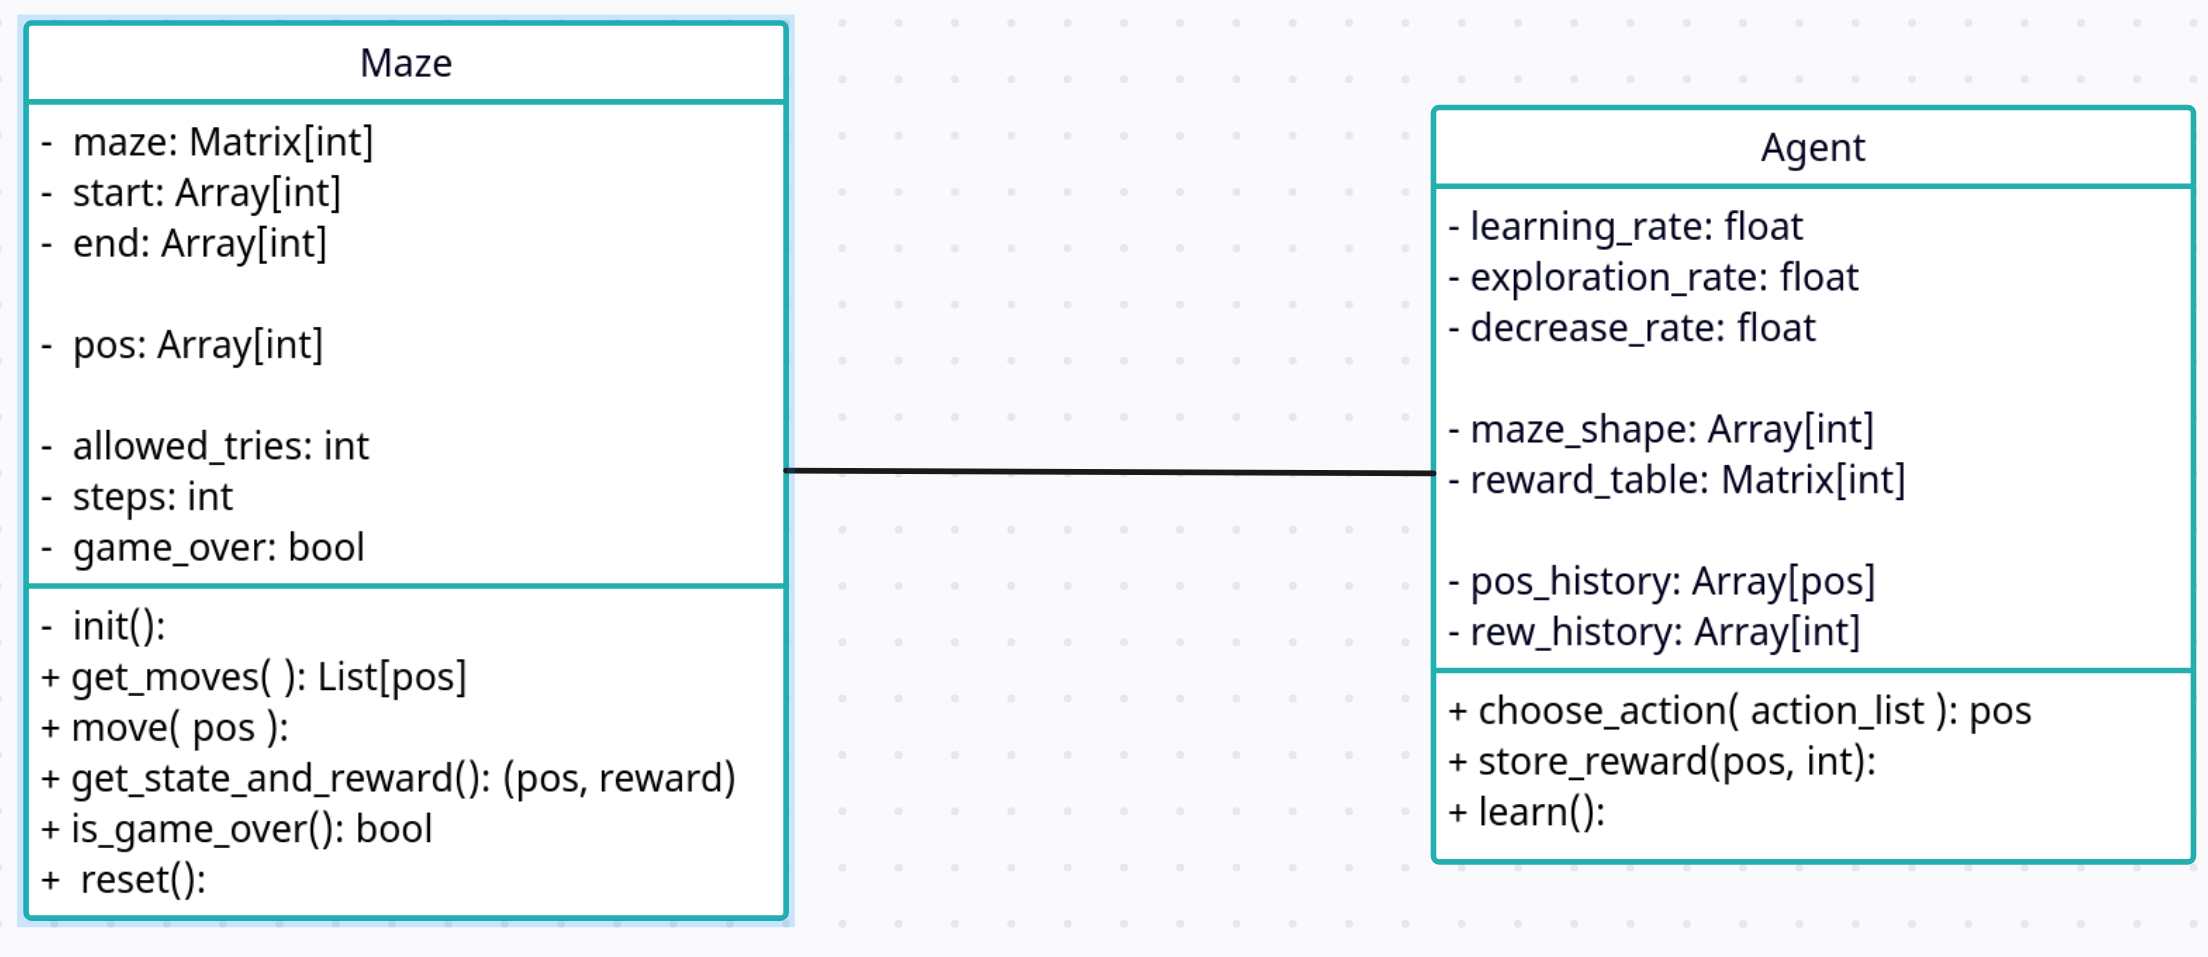
\includegraphics[width=0.9\textwidth]{class_diagrams.png}
    \caption{Class diagrams of the \texttt{Maze} and the \texttt{Agent}}
    \label{fig:class_diagrams}
\end{figure}

\subsection{Agent}

The implementation of the agent is more interesting in the context of
reinforcement learning.
The agent can be initialized with 3 different parameters all constrained on the
interval $[0,1]$:
\begin{enumerate}
    \item The learning rate $\alpha$,
    \item The exploration rate $\epsilon$ and
    \item The decrease rate $\gamma$.
\end{enumerate}
At the beginning the agent creates a reward matrix ($G$-table).
This matrix is used to map each position within the maze to an expected
cumulative reward $G_\mathrm{pos}$. This matrix is initialized with zero.
During one game (episode) the agent will store the sequence of positions (i.e.
his path) and the respective rewards associated with each position. It is only
after one game that he will learn. Let's take a closer look at this.

\subsubsection{Agent's \texttt{learn} method}
\label{sec:learn}
When the agent finishes a game, either by exceeding the step limit or by finding
the exit of the maze, he will try to learn from that game.
Figure (\ref{fig:learning}) illustrates the behavior.
The agent starts at the end of his path. He then computes the cumulative reward
along the path $G_\mathrm{path}$. In this simple case, as the reward is always
-1, the cumulative reward will measure the distance along the path towards the
end (with a negative sign). As such the maximization of cumulative rewards means
finding the shortest path. After computing the value $G_\mathrm{path}$ for a
given position, the stored value in the $G$-table of that position will be
adjusted:
\begin{equation}
    G_\mathrm{pos} = G_\mathrm{pos} + \alpha(G_\mathrm{path} - G_\mathrm{pos})
    \label{eq:learning}
\end{equation}
The agent will add a percentage (depending on the learning rate $\alpha$) of the
deviation between the observed cumulative reward ($G_\mathrm{path}$) and the
expected cumulative reward ($G_\mathrm{pos}$) to the expected cumulative reward.
In simpler words: \textit{the agent adjusts its expected reward towards the
observed reward}.
Lastly the agent will decrease its learning rate by multiplying it with the
decrease rate:
\begin{equation}
    \alpha = \alpha \cdot \gamma
\end{equation}
This ensures a decrease of $\alpha$ with time and thus more exploitation of the
gained knowledge about the maze. We thus \textit{hope} the agent converges on a
(good) solution.
After having understood how the agent learns his entries of the reward
table, let's look at how he uses his knowledge in order to choose his next move.

\begin{figure}
    \centering
    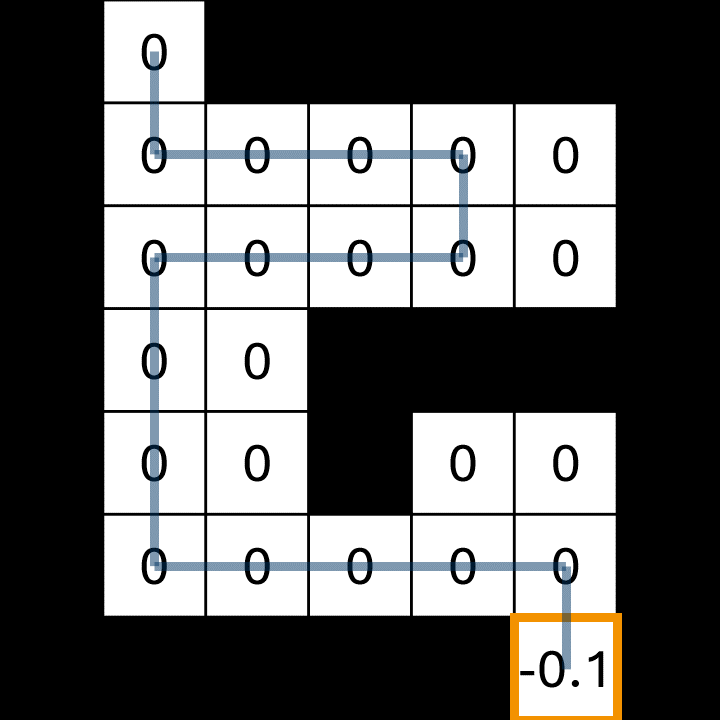
\includegraphics[width=0.3\textwidth]{learning/learning_1.png}
    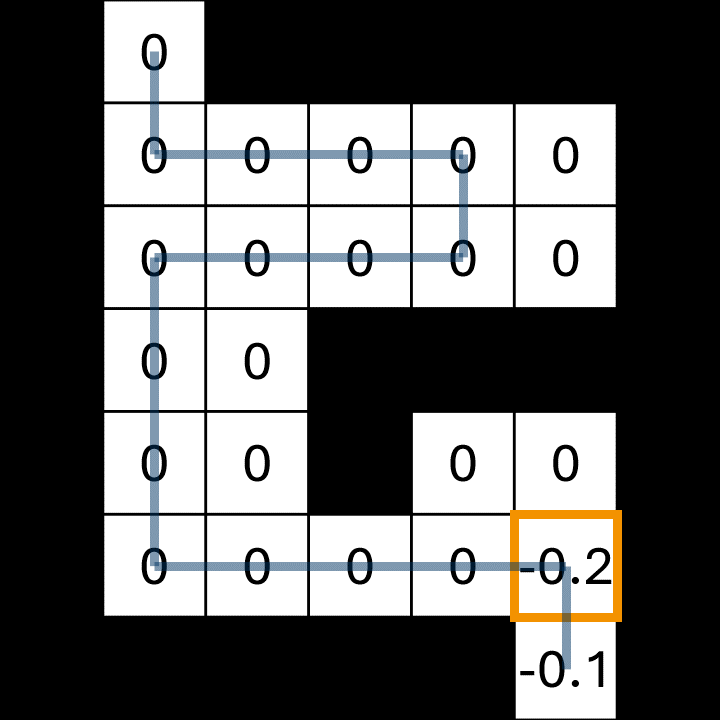
\includegraphics[width=0.3\textwidth]{learning/learning_2.png}
    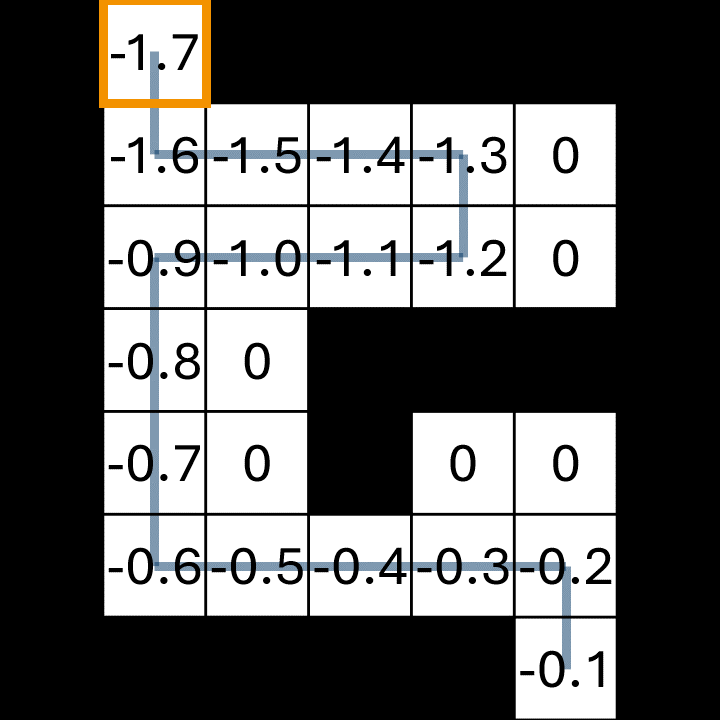
\includegraphics[width=0.3\textwidth]{learning/learning_end.png}
    \caption{
        Illustration of the learning process after the first game. Before the
        first game the agent's reward matrix is initialized with zeros.
        The agent follows the path backwards, computes the cumulative reward
        along the path ($G_\mathrm{path}$) and then learns according to formula
        (\ref{eq:learning}) with a value of $\alpha = 0.1$.\\
        \textit{Left:} Last step: 
        $reward = -1 \Rightarrow G_\mathrm{path} = -1 \Rightarrow 
            G_\mathrm{pos} = -0.1$ \\
        \textit{Middle:} Second last step: 
        $reward = -1 \Rightarrow G_\mathrm{path} = -2 \Rightarrow 
            G_\mathrm{pos} = -0.2$ \\
        \textit{Right:} $17^{th}$ last step: 
        $reward = -1 \Rightarrow G_\mathrm{path} = -17 \Rightarrow 
            G_\mathrm{pos} = -1.7$
    }
    \label{fig:learning}
\end{figure}

\FloatBarrier

\subsubsection{Agent's \texttt{choose\_action} method}
\label{sec:choose_action}

The \texttt{choose\_action} method can be explained rather quickly:
Usually the agent will follow a "greedy" algorithm, meaning he chooses the
action that maximises his (immediate) cumulative reward.
Standing at some position he will ask the environment for the possible moves
(actions). He will then evaluate the expected cumulative reward for each move.
The move resulting in the highest cumulative reward will be chosen.
Every once in a while however (tuned by the exploration rate $\epsilon$) he will
instead choose his move randomly. This modified approach is the called an 
\textit{Epsilon-Greedy Algorithm} \cite{eps_greedy} also known from the 
\textit{Multi-Armed Bandit Problem}.

\begin{figure}[htbp]
    \centering
    \animategraphics[width=0.3\textwidth, 
                     autoplay,
                     loop]{1}{choose_action/choosing-}{0}{12}
    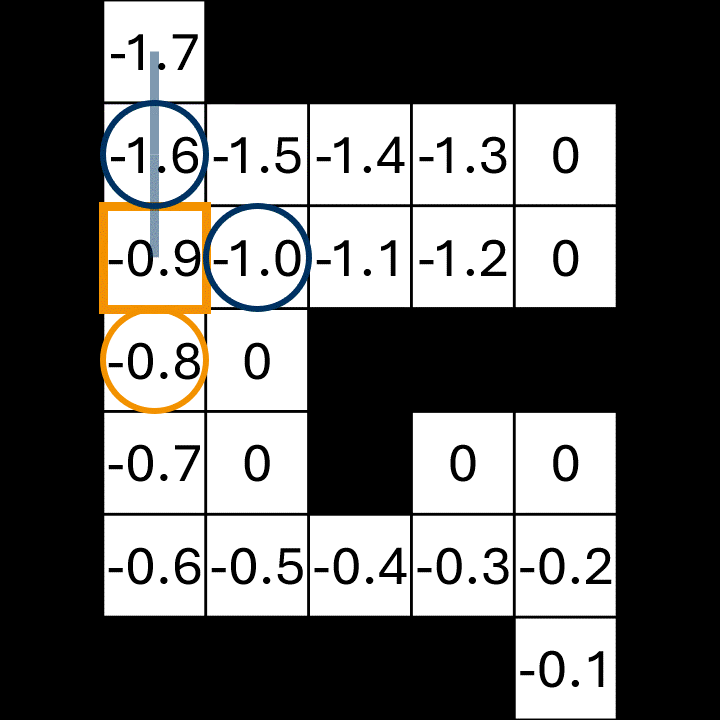
\includegraphics[width=0.3\textwidth]{choose_action/choosing-6.png}
    \caption{
        Illustration of how the agent chooses his action. Orange box: position
        of the agent, circles: possible moves to take, orange circle: selected
        move. The exploration part of the algorithm is not shown.\\
        \textit{Left:} Animation showing the agent and how he chooses his
        actions \\
        \textit{Right:} Chosen action for the third step 
        (if animation doesn't play)
    }
    \label{fig:choosing}
\end{figure}

\subsection{The training flow}
\label{sec:training}

In order to understand the whole process of training better, lets shortly cover
the training flow. A (minimal) version is shown in listing (\ref{lst:train}).
First important parameters like $\alpha$, $\epsilon$, $\gamma$ as well as 
\texttt{N\_iters}, the number of episodes for learning, are set. The maze and
the agent get initialized. In a loop the agent plays the game \texttt{N\_iters}
times. Each game is played as follows: The agent asks for the moves and chooses
one of them. After the execution of the action, the agent stores the reward
provided by the maze. This continues until the game is over either because the
agent reached the end of the maze, or because he exceeded the maximum amount of
steps he may take. After each game the agent invokes his \texttt{learn} method
described in section (\ref{sec:learn}). Before the next game the maze gets
reset to its initiallization state.

\lstinputlisting[
    style=python,
    label={lst:train},
    caption = {
        The training routine for the agent.
        Describtion in section (\ref{sec:training})
    }
]{train_stripped.py}

% --- Performance ----------------------------------------------------------------------------------
\section{Learning Parameters}
\label{seq:parameters}

Now follows an investigation of how the agent performs. Figure 
(\ref{fig:big_maze_decrease_rate}) shows the agents solution after 500
iterations of learning. We can clearly see the impact of the decrease rate
$\epsilon$. If $\epsilon$ is a relatively low value (0.95) the exploration rate
reduces so quickly that the agent is basically unable to find the exit of the
maze. Raising the value to 0.99 we can see that the agent is able to
solve the maze. The transition between solved and unsolved however is very
sudden, indicating, that finding the solution can be somewhat a matter of luck.
If we raise $\epsilon$ even further, we can see that he starts to succeed
however to reliably find the solution it took a little longer that in the
previous case.
With the discussion about the decrease rate $\gamma$ we can also conclude the
discussion about the exploitation rate $\epsilon$. Both parameters control the 
how extensively the agent explores the environment. The exploration rate however
is simply a scalar multiplicator whereas the decrease rate determines the speed
with which the exploration rate decays exponentially and is thus a more
important parameter. Maybe the names are misleading and could be chosen better.

\begin{figure}[htbp]
    \centering
    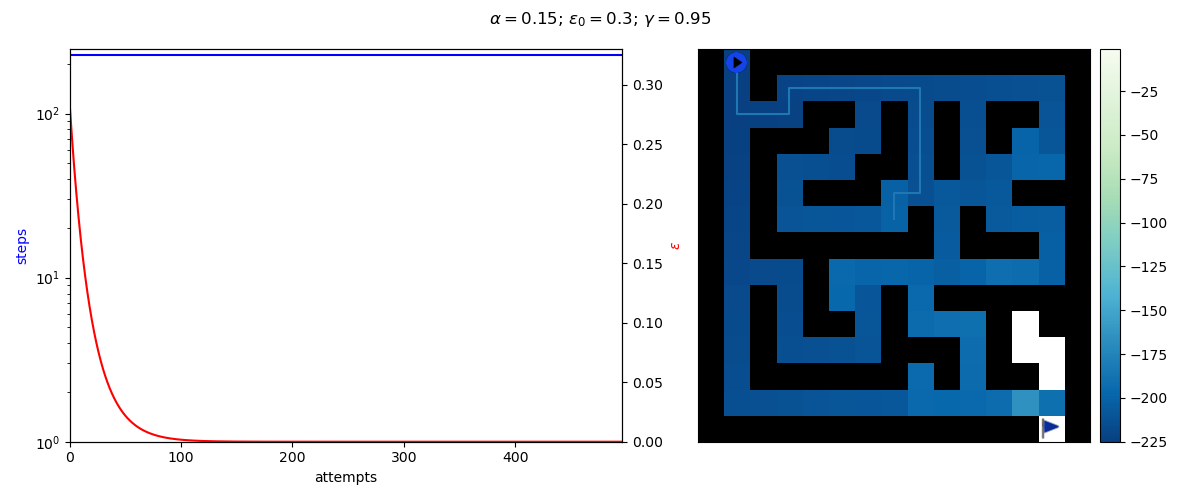
\includegraphics[width=0.9\textwidth]{parameters/big_mazeN500_lr0.15_er0.30_dr0.95000.png}
    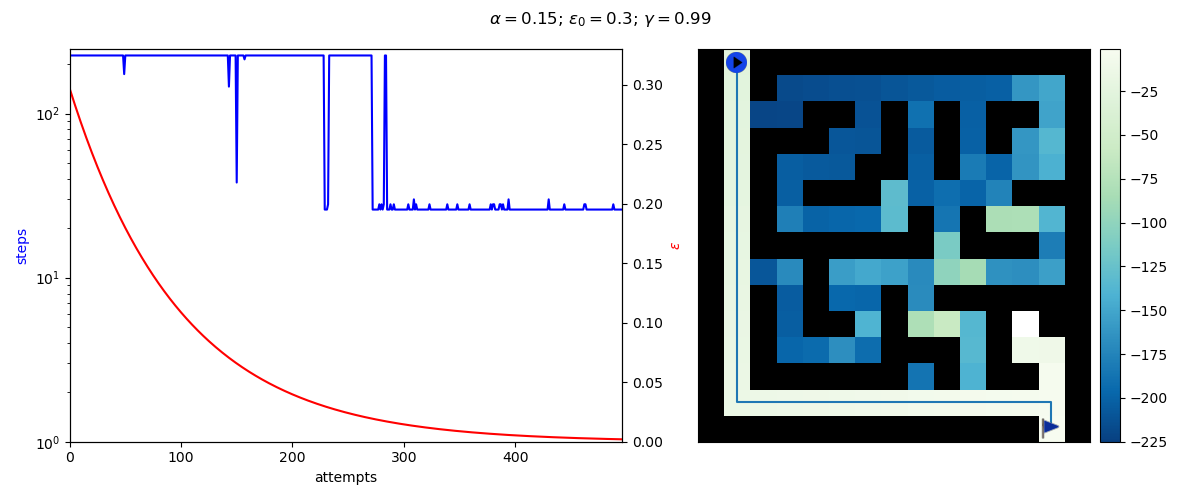
\includegraphics[width=0.9\textwidth]{parameters/big_mazeN500_lr0.15_er0.30_dr0.99000.png}
    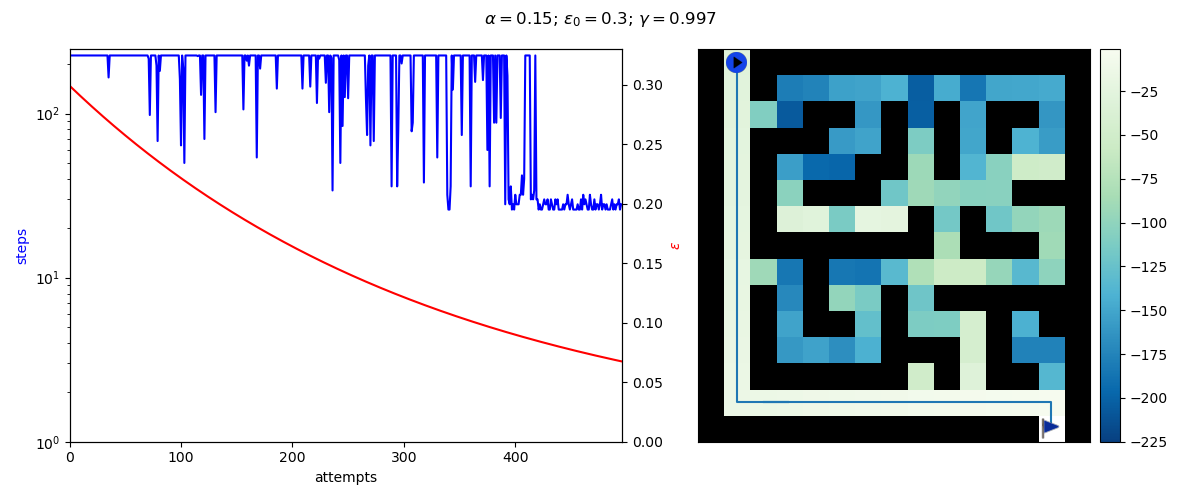
\includegraphics[width=0.9\textwidth]{parameters/big_mazeN500_lr0.15_er0.30_dr0.99700.png}
    \caption{
        The training of an agent on a maze with 500 iterations.
        Each row corresponds to a differen decrease rate ($\epsilon$) (0.95,
        0.99 and 0.997 from top to bottom). \\
        \textit{Left column:} The number of steps it takes the agent to finish a
        game. It is limited to 255 attempts (blue). The exploration rate 
        ($\epsilon$) in red. \\
        \textit{Right column:}  The maze (black walls) and the $G$-table
        (colored fields) of the agent after the last attempt. The path of the
        last attempt as blue line.
    }
    \label{fig:big_maze_decrease_rate}
\end{figure}

Going further to the learning rate $\alpha$. It also showed less effect on the
overall performance than the decrease rate. Figure 
(\ref{fig:big_maze_learning_rate}) shows the last plot of figure
(\ref{fig:big_maze_decrease_rate}) but with a decreased learning rate
of $\alpha = 0.05$. I suspect the learning rate to be more relevant in more
complex systems. For such small systems as shown here the $G$-table entries are
not overall good approximations of the distance towards the exit of the maze.
As such the agent is not concerned with learning the correct values but once he
has found a way he will continously choose this same path. Along this path the
the entries of the $G$-table \textit{will} converge and thus \textit{are}
good approximations, but this only happens \textit{after} the agent has already
found the way. In this sense I suspect the importance of $\alpha$ to grow when
the options of different paths increas and the relative difference along those
paths decreases. With this I want to conclude the discussion about the
parameters and turn to a different topic with wich I delt more.
This is the design of the two core algorithms: the learning and the selection
of the action.

\begin{figure}[htbp]
    \centering
    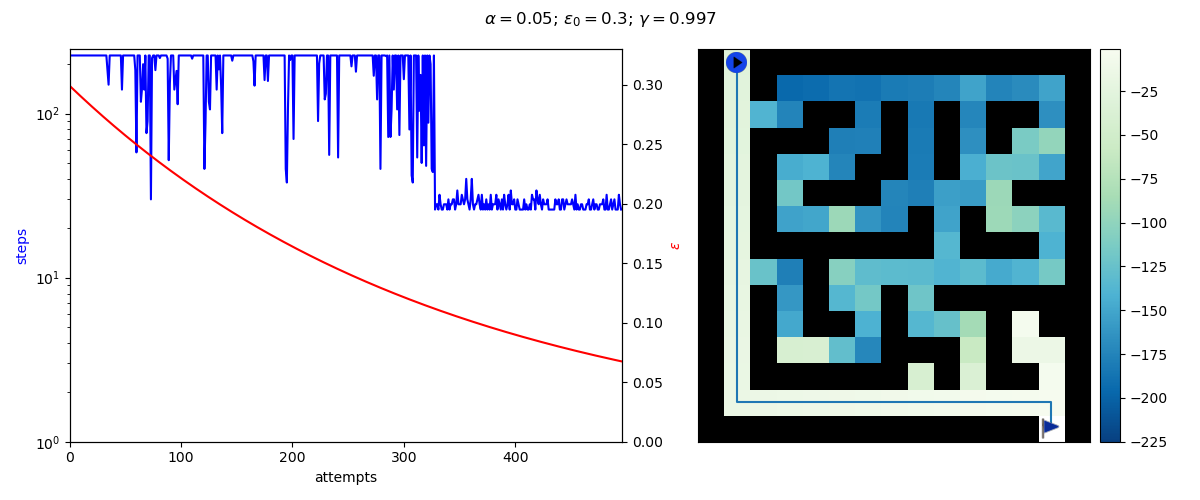
\includegraphics[width=0.9\textwidth]{parameters/big_mazeN500_lr0.05_er0.30_dr0.99700.png}
    \caption{
        The training of an agent on a maze with 500 iterations.
        Training parameters are set to $\alpha = 0.05$, $\epsilon_0 = 0.3$ and
        $\gamma = 0.997$. In comparison with figure
        (\ref{fig:big_maze_decrease_rate}) bottom only the learning rate is
        reduced. This shows litte effect on the overall outcome.
    }
    \label{fig:big_maze_learning_rate}
\end{figure}

\FloatBarrier
\section{Algorithmic Improvements}
\label{seq:improvements}

During different training runs I realized one thing. Often the agent does not
walk very far at all. Sometimes he steps into a \textit{hallway} but immediately
steps back out other times simply runs back and forth. Figure
(\ref{fig:choose_action2}) shows two examples of the agent's behavior.

\begin{figure}[htbp]
    \centering
    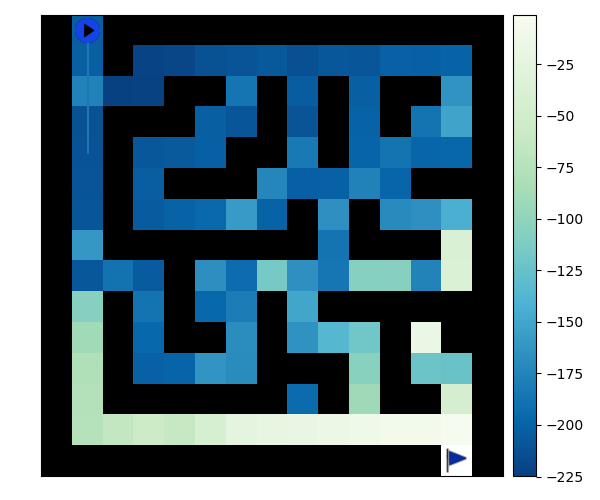
\includegraphics[width=0.3\textwidth]{algorithms/bad_exploration_example.png}
    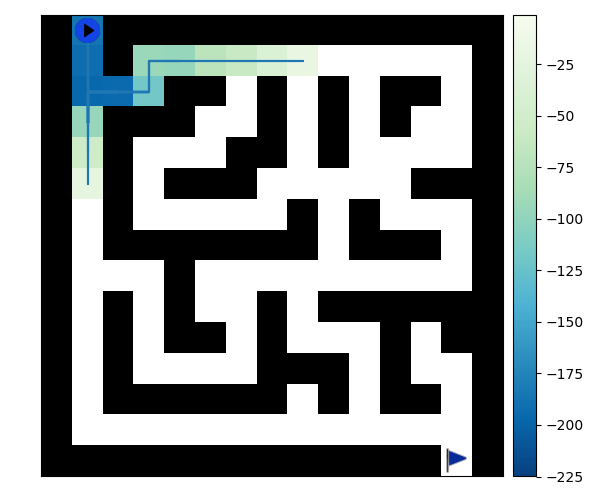
\includegraphics[width=0.3\textwidth]{algorithms/choose_big_maze_N1_lr0.15_er0.30_dr0.99000.png}
    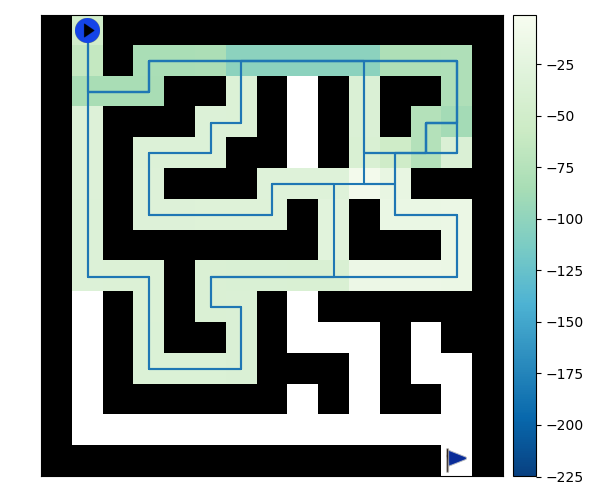
\includegraphics[width=0.3\textwidth]{algorithms/choose2_big_maze_N1_lr0.15_er0.30_dr0.99000.png}
    \caption{
        \textit{Left:} A particular extreme example of the agent beeing stuck
        running only back and forth. This even happend after training. \\
        \textit{Middle:} A typical first attempt of the agent on a new maze.
        The exploration territory is quite small. \\
        \textit{Right:} After the new \texttt{choose\_action} algorithm the
        agent exploration territory increased significantly.
    place.}
    \label{fig:choose_action2}
\end{figure}

\subsection{Improved \texttt{choose\_action} Algorithm}
\label{sec:choose_action2}

My approach to solving this problem was quite simple: after selecting an action
the algorithm checks if this action results in stepping on the field he came
from. If so, he also checks if can choose from more than on action.
If it is the only action available the agent is in a dead end. Thus, it is okay
to go back and he will stick with the action. If however he has more than one
option, he disregars the selected option and chooses again.
This simple adaptation of the algorithm proved to be a drastic improvement in how
quickly the agent explores the territory.

\subsection{Improved Learning Algorithm}
\label{sec:improved_learn}

Another problem appears when the agent tries to learn from an unsuccessful
attempt. Figur (\ref{fig:false_high}) shows such an occurence. To understand why
this might be a problem, the same figure also shows an example of how the
cumulative rewards might look like. We obsere that for some fields multiple
cumulative rewards can exist. Instead of learning the more "conservative" option
(i.e. the lower reward) the agent first learns the higher value and the later
during the learning algorithm he revisits the same Fields and learns the lower
option. Another option that showed slight improvements (especially without the
improved \texttt{choose\_action} algorithm) is to only select the lower value of
the two and only learn from that. The last figure (\ref{fig:learn_comp}) shows
the performance on a bigger maze. For both plots the improved
\texttt{choose\_action} version is use, only the lower one uses the ned learning
variant. As can be seen the new learning varant improves the speed with which
a solution is found. With only the new learning algorithm the agent is
significantly slower, without any improvements I could not make the agent find
any solution.

\begin{figure}[htbp]
    \centering
    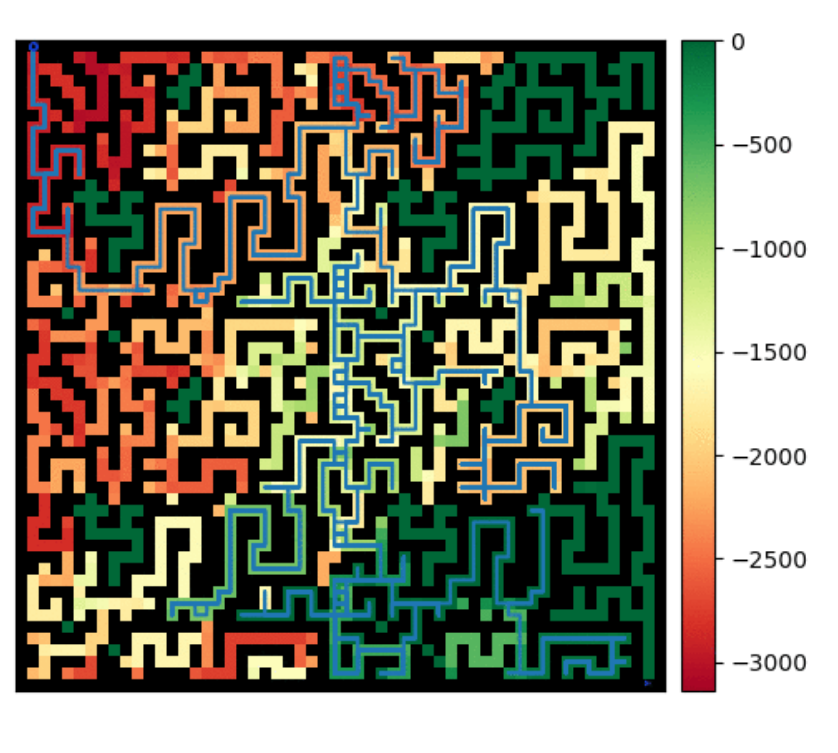
\includegraphics[width = 0.32\textwidth]{algorithms/false_high_1.png}
    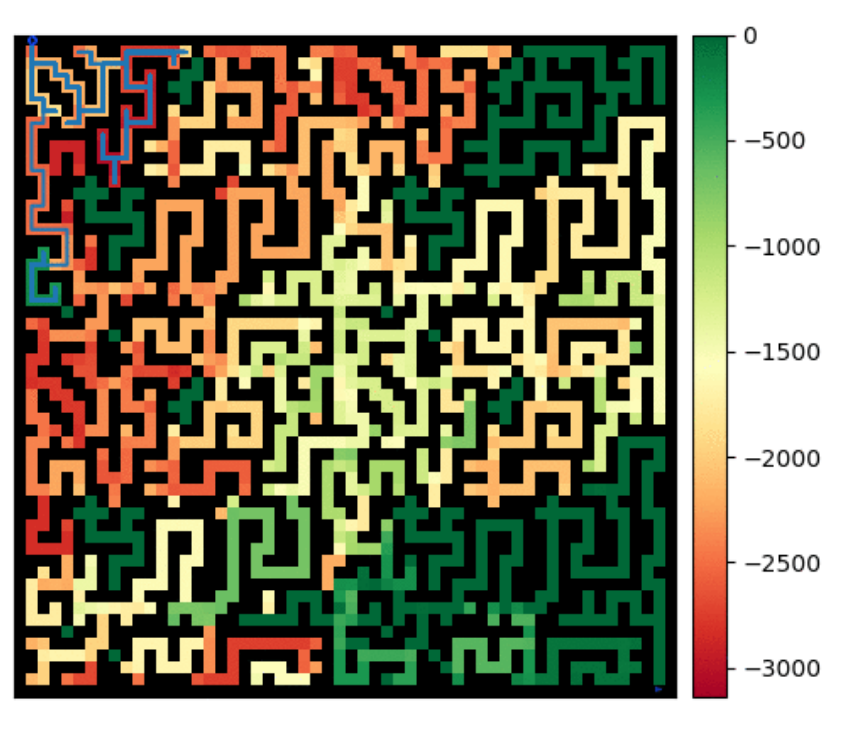
\includegraphics[width = 0.32\textwidth]{algorithms/false_high_2.png}
    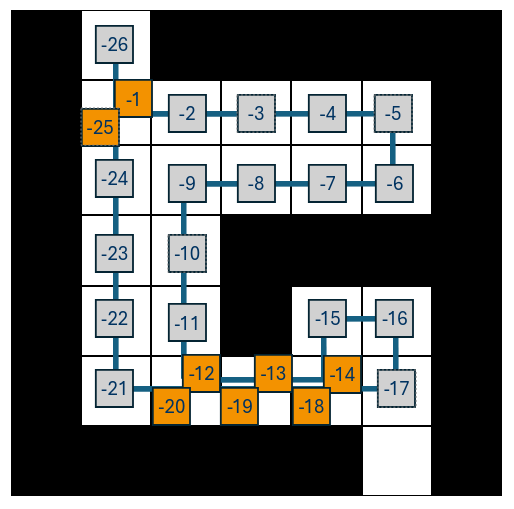
\includegraphics[width = 0.28\textwidth]{algorithms/new_rewards.png}
    \caption{
        The agent tries to learn from an unsuccessful attempt.\\
        \textit{Left:} Reward matrix prior to the attempt.\\
        \textit{Middle:} Attempt and the reward matrix after the attemt.\\
        When focusing on the upper left corner we can see, that the entries
        within the reward matrix increased, even though the agent did not find
        any connection between them and the exit of the maze. \\
        \textit{Right:} A example of how the cumulative rewards along an
        unsuccessfull path could look like. Most likely there are fields for
        wich multiple cumulative rewards exist. Originally the agent would learn
        from both these values, effectively learning the mean value.
    }
    \label{fig:false_high}
\end{figure}

\begin{figure}[htbp]
    \centering
    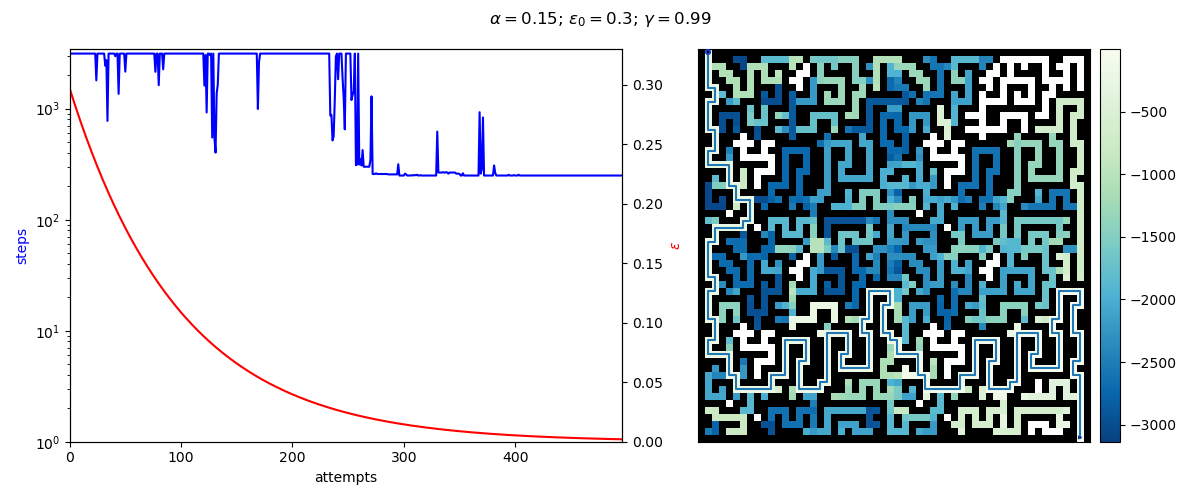
\includegraphics[width=0.9\textwidth]{algorithms/learn_choose2_very_very_big_mazeN500_lr0.15_er0.30_dr0.99000.png}
    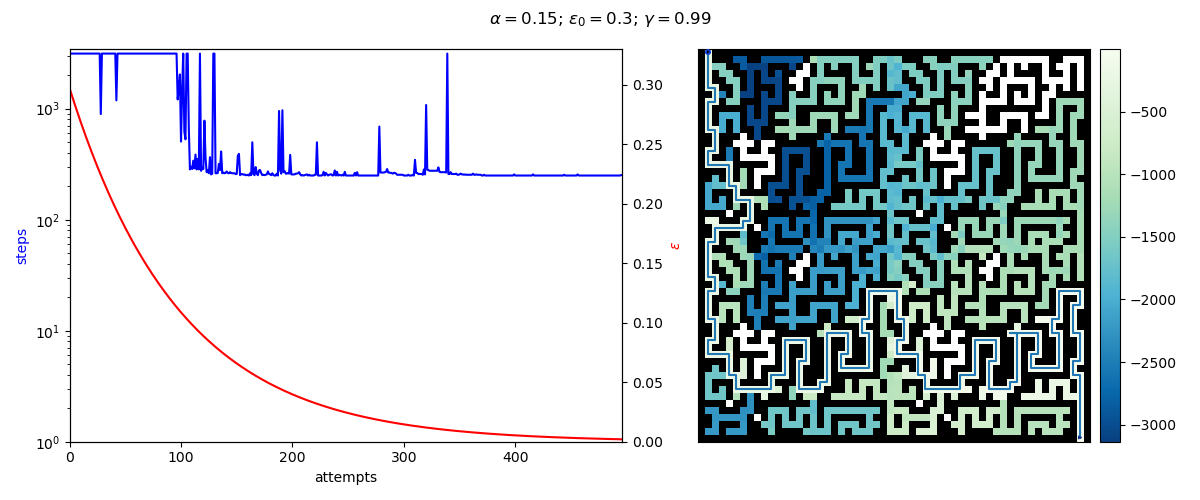
\includegraphics[width=0.9\textwidth]{algorithms/learn2_choose2_very_very_big_mazeN500_lr0.15_er0.30_dr0.99000.png }
    \caption{The agent solving a larger maze. \\
    \textit{Top:} The agent only uses the improved \texttt{choose\_action}
    algorithm. \\
    \textit{Bottom:} The agent additionly employs the new learning algorithm.
    This results in better performance.
    }
    \label{fig:learn_comp}
\end{figure}

\FloatBarrier
% --- CONCLUSIONS ----------------------------------------------------------------------------------
\section{Conclusions and Outlook}
\label{sec:conclusions}

Finally let's shortly discuss the learnings.
I introduced a machine learning paradigm called reinforcement learning.
With the example of a maze i constructed an algorithm which could solve small
mazes. After investigation of the effect of the different parameters I concluded
that the most important parameter is the decrease rate $\gamma$. Additionly I
was able to find to adaptations of the algorithms presented in the tutorial
which enabeled me to tackle much bigger mazes than previously.

What I haven't covered yet are any adaptations to the general problem. As witten
in our case the maze always return a reward of -1. This seems limiting. An easy
adaptation would be to introduce different Fields within the maze. One could
imagine the along some paths the ground is more sandy and thus movement take
more effort or a puddle has to be crossed. This should in principle be only a
slight modification, this time on the side of the maze. There are many more
problems that could and will be solved by reinforcement learning so let's see
what is to come.


% --- END OF CONTENT -------------------------------------------------------------------------------
\clearpage
\vfill

% --- REFERENCES -----------------------------------------------------------------------------------
\section{References}
\printbibliography
\newpage

% --- DECLARATION ----------------------------------------------------------------------------------
% --- DECLARATION ----------------------------------------------------------------------------------
\section*{Declaration}
\thispagestyle{empty}
Hereby I declare, that this report is fully written
by myselve and any necessary sources are referenced.

\begin{tabular}{@{}p{2.5in}p{2.5in}@{}}
 \\[5\bigskipamount]
  \dotfill & \dotfill \\
   \ \  Jakob Floß  & \ \ Date \\[5\bigskipamount]
  \centering
\end{tabular}

\clearpage

% \appendix

% \definecolor{keywords}{rgb}{0.80, 0.25, 0.18}
\definecolor{comments}{rgb}{0.24,0.48,0.48}     % comments
\definecolor{codegray}{rgb}{0.5,0.5,0.5}
\definecolor{codepurple}{rgb}{0.58,0,0.82}
\definecolor{backcolour}{rgb}{0.85,0.85,0.85}
\definecolor{aqua}{cmyk}{0.65,0,0.23,0}         % class types
\definecolor{lavender}{cmyk}{0,0.42,0,0.1}      % conditionals
\definecolor{self}{rgb}{76,0.53,0.06}           % conditionals


\lstdefinestyle{python}{
    language=Python,
    frame=tbl,
    backgroundcolor=\color{backcolour},  
    basicstyle=\ttfamily\scriptsize,
    keywordstyle=\color{keywords},
    % identifierstyle=\color{blue},
    stringstyle=\color{codepurple},
    commentstyle=\color{comments},
    numberstyle=\tiny\color{codegray},
    breakatwhitespace=false,         
    breaklines=false,                 
    captionpos=b,                    
    keepspaces=true,                 
    numbers=left,                    
    numbersep=5pt,                  
    showspaces=false,                
    showstringspaces=false,
    showtabs=false,                  
    tabsize=4,
    emph={self},
    emphstyle =\color{self}
}

% \lstset{style=python_style}

% \section{\texttt{train.py}}
% \lstinputlisting[style=python]{../train.py}
% \section{\texttt{agent.py}}
% \lstinputlisting[style=python]{../agent.py}
% \section{\texttt{maze.py}}
% \lstinputlisting[style=python]{../maze.py}

\end{document}